\documentclass{beamer}
\mode<presentation> {
\usetheme{Madrid}
}
\usepackage{graphicx} % Allows including images
\usepackage{booktabs}
\RequirePackage[utf8x]{inputenc} % Allows the use of \toprule, \midrule and \bottomrule in tables
\usepackage{amsmath}
\usepackage{dsfont}
\usepackage{amsthm}
\newtheorem{remark}{Remark}


%----------------------------------------------------------------------------------------
%	TITLE PAGE
%----------------------------------------------------------------------------------------

\title{Introduzione all'Ingegneria Finanziaria}
\author{\textbf{Vincenzo Eugenio Corallo}}


\institute[DSE Sapienza] 
{	
	\footnotesize{vincenzo.corallo@uniroma1.it}\\
	\bigskip
	\bigskip
	
\includegraphics[width=20 mm]{Uniroma1.png} \\ 	
	\bigskip
	Doctoral School of Economics (DSE)
}
\date{\today} 

\begin{document}

\begin{frame}
	\titlepage % Print the title page as the first slide
\end{frame}



%----------------------------------------------------------------------------------------
%	PRESENTATION SLIDES
%----------------------------------------------------------------------------------------


\begin{frame}
\frametitle{Table of contents}
	\footnotesize{\tableofcontents}
\end{frame}

\section{Richiami di Finanza Matematica}
\begin{frame}
		
\end{frame}

\section{Technical background, introduction to CCR and \textit{valuation adjustments} and main contributions of the work}

\begin{frame}
\Huge{\centerline{Introduction}}
\end{frame}
\begin{frame}
\frametitle{Counterparty Credit Risk (CCR) definition}

	\textbf{Counterparty Credit Risk (CCR)} is the risk which economic agents face due to the possible default of their over the counter (OTC) counterparts occurring prior to the full compliance of contractual payments. \\~\\
 	
	We have learned from the global financial crisis,
	that no banking or corporate entity can be  
	any more considered entirely default-free. In other words, CCR \textit{bilaterally} affects OTC derivatives trades.\\~\\
	
	Differently from loans, in the case of derivatives the future exposures toward the counterpart are not known today. Therefore, potential \textbf{future losses are stochastic}.

\end{frame}

\begin{frame}
\frametitle{XVA and consequences in Fair Valuation}
	Economic reasoning suggests that the fair value of a CCR risky contract has to be lower than the one of an identical default-free contract. \\~\\

	The deviation between these two prices is known as the \textbf{Total Valuation Adjustment (XVA)\footnote{In the acronym, the "X" denotes a variable letter depending on the specific valuation adjustment to be analysed.}} and is a correction on the fair value due to the presence of default risk.  \\~\\
	
	In terms of \textit{fair valuation}, the XVA represents the \textbf{fair price of Counterparty Risk}.

\end{frame}

\begin{frame}
\frametitle{No risk-free funding and valuation adjustments}

	In the economic perspective, \textbf{funding costs} over the risk-free rate might be viewed as a friction of the post-crisis financial market where no agent can borrow at the risk-free rate any more.\\~\\

 	The \textbf{Funding Valuation Adjustments (FVA)} is defined as the expected cost of financing the hedging portfolio. \\~\\

	Similar reasoning can be extended to the \textbf{Initial Margin Valuation Adjustment (MVA)}, which is basically the expected cost of financing the initial margin.  \\~\\
	
	The \textbf{initial margin (IM)} is required by both the Standard Collateral Support Annex (SCSA) or by a Central Clearing Counterparty (CCP), in order to cover additional risks on top of those covered by variation margins (VM).
\end{frame}

\begin{frame}
\frametitle{Main contributions of my thesis}
\textbf{Chapter 1}:
\begin{itemize}
	\item Derivation of a \textbf{model independent BVA formula}
	\item Application of a \textbf{hybrid Fourier-Monte Carlo numerical technique}
\end{itemize}

\textbf{Chapter 2}:
\begin{itemize}
	\item Arrangement of \textbf{FVA outside fair valuation}
	\item Estimation of \textbf{FVA bid/ask spread widening} and relations with funding strategies
	\item Extension of Burgard-Kjaer (2011b) results
\end{itemize}

\textbf{Chapter 3}:
\begin{itemize}
	\item Inclusion of \textbf{stochastic recovery rates}
	\item Model risks implied in deterministic recoveries
\end{itemize}
\end{frame}

\begin{frame}
\frametitle{Theoretical Framework}

	\textbf{Default model}: in this work the random default time is modelled through the structural approach proposed in the classic work of \textbf{Black and Cox} (1976), \textit{i.e the bankruptcy is defined as the first time the firm equity value hits a predetermined lower barrier}.
	The focus on equity, instead of the firm value, is motivated by its status of \textit{tradable} asset. 
    \\~\\
	\textbf{Credit and Market model}: as in Ballotta et al. (2015), in this work it is proposed a \textbf{\emph{time-changed} Lèvy process} as underlying source of both market and credit risks. The adoption of a pure jump stochastic process is motivated, among other reasons, by its superior capability to replicate non null short-term default probabilities unlike the Geometric Brownian Motion (GBM). 	Moreover, Lèvy processes can replicate implied volatility surfaces without overstress model parameters and can accommodate for jumps. The presence of jumps in the path of risky assets implies the market is in general \textbf{incomplete}, see Cont and Tankov (2004).
\end{frame}



\begin{frame}
\frametitle{Model setup}
	In a bilateral counterparty risk perspective, let me introduce two \textbf{defaultable} counterparts involved in a OTC derivative deal denoted by the investment bank B (the dealer) and its client C (which might be a corporate firm or another bank).\\~\\
	
	The market is modelled through the assignment a \textbf{filtered probability space} $(\Omega,\mathbb{Q},\mathcal{G}_t)$ in which $\Omega$ is the set of possible events, $\mathbb{Q}$ is some \emph{risk-neutral} martingale measure and the enlarged filtration is defined as $\mathcal{G}_t := \mathcal{F}_t \vee \mathcal{H}_t$. \\~\\

	$ \{ \mathcal{F}_t \}_{0 \leq t \leq T}$ is the reference filtration which contains all market information except of default events up to time $t$, while $ \{ \mathcal{H}_t \}_{0 \leq t \leq T}$ is the algebra $\sigma(\tau \wedge t)$ generated by default history. The random \emph{first-to-default} time is defined as $\tau  := \tau_{B} \wedge \tau_{C}$. 

\end{frame}

\begin{frame}
\frametitle{Introducing Lèvy processes}
	An infinitely divisible \emph{càdlag} (right continuous with left limit) stochastic process $\{ X_t \}_{0 \leq t \leq T}$ defined on the filtered probability space $(\Omega,\mathbb{Q},\mathcal{G}_t)$ is said to be a Lèvy process if it %is stochastically continous and 
  	presents stationary and independent increments. In general, the distribution of a Lèvy process can allow for:
  	\begin{itemize}
  		\item \textbf{jumps}
  		\item non-zero \textbf{skewness} and \textbf{excess kurtosis}
  	\end{itemize}  
  	
	For the class of Lèvy processes, it is often impossible to determine analytically the transition density but their characteristic function $\phi$, is always available in closed form thanks to the well known \textbf{Lèvy-Khintchine representation}:

	\begin{equation}
	\phi_{X}(u;t)= \mathbb{E} \lbrack e^{\imath u X(t)} \rbrack = e^{t \varphi_{X}(u)}, \quad u \in \mathbb{R}
	\end{equation} 
	
	where $\varphi_{X}(u)$ is the \emph{characteristic exponent} of $X_{t}$ of the Fourier parameter $u$.
\end{frame}

\begin{frame}
\frametitle{The Normal Inverse Gaussian (NIG) process}
	The \textbf{Normal Inverse Gaussian (NIG)} is a \emph{pure jump} Lèvy process obtainable by subordinating a Brownian Motion to an independent Inverse Gaussian Process $IG(t)$. The NIG process, similarly to others obtainable by \textbf{subordination}, is said to be a \emph{time-changed} Lèvy process: in other words, it is indexed to a \textit{stochastic clock}. The NIG process presents the following form:

	\begin{equation}
		X(t) = \mu IG(t) + \sigma W_{IG(t)}
	\end{equation}

	The \textbf{characteristic exponent} in the case of NIG process is:

	\begin{equation}
		\varphi_{X}(u) =  \frac{1- \sqrt{1-2 \imath \theta \kappa + u^{2}\sigma^{2}\kappa}}{\kappa}
	\end{equation}

	where $\imath$ is the imaginary unit and as for the \textbf{meaning of parameters }is concerned, $\theta \in \mathbb{R}$ describes the sign of the skewness of the process distribution, $\sigma > 0 $ is the volatility parameter and $\kappa > 0$ controls the excess kurtosis of the distribution.
\end{frame}

\begin{frame}
\frametitle{Meaning of the brownian subordination}
	Building Lèvy processes through subordination is particularly convincing from the economic point of view, since \textbf{time-changing} might be interpreted as the \textbf{switch from calendar time to business time}. This relates to the idea  of asset prices mainly driven by the relevant news whose both arrival time and impact on the market is random.\\~\\

	Interestingly, the empirical evidence suggests that gaussianity of asset returns seems to be recovered under such trading time. \\~\\

\end{frame}

\begin{frame}
\frametitle{Risk-neutral dynamics}
	In this framework the NIG process $X_{t}$ is the relevant \emph{risk driver} for the uncertain dynamics of the underlying asset $S_{t}$, whose price at time $t$ under the risk neutral measure $\mathbb{Q}$ is:

	\begin{equation}\label{price}
		S_{t}=S_0e^{(r-q-\varphi_{X}(-\imath))t+X(t)}
	\end{equation}

	where $r>0$ is the risk-free rate\footnote{In current market environment this is a theoretical unobservable rate. What can be done is approximate it through overnight rates.} and $q>0$ is the constant \emph{dividend yield} paid by the underlying stock (being zero for commodity assets). \\~\\

	From an empirical point of view, since energy commodities prices are much more volatile than stocks and present significant discontinuities in their path, they are  well suited to be modelled by a Lèvy process.
\end{frame}

\begin{frame}
\frametitle{Credit events}
	Suppose equation \ref{price} describes the equity value of firms $ \{B,C\}$ in addition to that of the underlying commodity asset. Then, the default of the firm is modelled as first passage time at the level of the barrier:


	$$\tau_{i}:= \inf \{ t \in (0,T] : S_{i}(0)e^{(r-q_{i}-\varphi_{X_{i}}(-\imath))t+X_{i}(t)} \leq K_{i}\}$$

	$$\text{or equivalently,}$$


	$$=\inf \{ t \in (0,T] : X_{i}(t) \leq \log{  \left(\frac{ K_{i} } {S_{i}(0)} \right)} - (r-q_{i}-\varphi_{K_{i}}(-\imath))t\}$$ 
	
	Let me define the default indicators $\{ D^{i}_t \}_{0 \leq t \leq T}$ denoting the occurrence of the respective credit events:
	$$D_{t}^i := \mathds{1}_{ \{ \tau_{i} \leq t \} }, \quad i \in \{B,C  \} $$

\end{frame}


\section{Chapter 1: Lèvy-based Structural Pricing of Bilateral Counterparty Credit Risk (CCR) }

\begin{frame}
	\Huge{\centerline{Chapter 1}}
\end{frame}

\subsection{Theoretical framework}

\begin{frame}
\frametitle{Close-out procedures: the ISDA Master Agreement}
	In presence of Counterparty Credit Risk it is used distinguish between $V(t,S)$, which denotes the economic value  at time $t$ of the \emph{default-free} derivative contract, and ${\hat{V}(t,S,D_{B},D_{C})}$, which denotes the value of a correspondent counterparty risky claim.  \\~\\
	
	In case of no default before the maturity of the contract, at time $T$ the buyer will receive or make the flow of contractual payments correspondent to the derivative payoff $\hat{\Phi}(S_{T})$, while the dealer earns the opposite cash flows $-\hat{\Phi}(S_{T})$. \\~\\

	According to \textbf{2002 ISDA Master Agreement} in case of premature default, the surviving counterpart would pay all its debt if it is \emph{out of the money} or, in case of being \emph{in the money}, it could claim just a recovery fraction of its credit.

\end{frame}

\begin{frame}
\frametitle{Bilateral Counterparty Credit Risk pricing}
	\newtheorem{prop}{PROPOSITION 1}
	\begin{prop}
	Let me denote by $\varepsilon_{t}$ the exposure toward the counterpart at time $t$. Suppose that in compliance with the \textbf{ISDA 2002 close-out agreements} at the stopping times $\tau_{C}$ and $\tau_{B}$, the following border conditions hold:
	
	\begin{equation}\label{ISDA}
	\begin{split}
		\hat{V}_{\tau_{C}} = R_{C}(\varepsilon^{+}_{\tau_{C}}) - \varepsilon^{-}_{\tau_{C}} \\
		\hat{V}_{\tau_{B}} =\varepsilon^{+}_{\tau_{B}}- R_{B}(\varepsilon^{-}_{\tau_{B}})
	\end{split}
	\end{equation}

	then, according to the Asset Pricing Theorem (APT) the \textbf{value at time $t$ of a counterparty-risky derivative claim} is:
	
	\footnotesize {
	\begin{equation}\label{BVA}
		\hat{V}_t= V_t -  \underbrace{\mathbb{E}_{t}[ \mathds{1}_{ \{ \tau = \tau_{C} \} } D(t,\tau_{C}) (\varepsilon_{\tau_{C}}^{+}- R_{C}(\varepsilon_{\tau_{C}}^{+}))]}_{CVA}+ \underbrace{ \mathbb{E}_{t}[ \mathds{1}_{ \{ \tau = \tau_{B} \} } D(t,\tau_{B}) (\varepsilon_{\tau_{C}}^{-}- R_{B}(\varepsilon_{\tau_{B}}^{-}))] }_{DVA}
	\end{equation} }

	\end{prop}
\end{frame}

\begin{frame}
\frametitle{The price of CCR: economic interpretation}
	By assuming that both the recovery functions take deterministically values in [0,1]:
	\begin{itemize}
		\item the \textbf{Credit Valuation Adjustment (CVA)} appears to be a call option with zero strike and random maturity issued on the uncollaterized exposure and represents the \textbf{expected loss on banks's credits} due to counterparty deafault risk.
		
		\item Conversely, the \textbf{Debt Valuation Adjustment (DVA)} appears to be a put option with zero strike and random maturity issued on the uncollateratized exposure and represents the \textbf{expected gain on bank's debts} due to its own default risk.
	\end{itemize}
\end{frame}

\subsection{Introduction of Fourier Pricing for calibration end exposures computation}

\begin{frame}
	\frametitle{Case study}
	
	Two firm have been involved in the numerical application: a representative bank, and a representative corporate firm. They are supposed negotiating OTC derivative claims issued on the most liquid energy commodity assets quoted in the Chicago Mercantile Exchange (CME), i.e. \textbf{crude oil} and \textbf{natural gas}. 
	Relying on the theoretical framework I have set up, the XVA metrics for vanilla energy commodities derivative have been estimated numerically. The analytic have been developed in \textbf{Python 2.7}. \\~\\


	From a computational point of view, since in general the distribution of Lèvy processes is not known in closed form, it is required the use of some Fourier pricing technique. The \textbf{Fourier Cosine Serie (COS) method}, proposed by Fang and Oosterlee (2008) has been chosen for both the calibration and exposures calculation because of its recognized better efficiency compared, for instance, to the \textbf{FFT} (Fast Fourier Transform), see Carr and Madan (1999) or the Convolution method (CONV), see Lord et al. (2008).
\end{frame}

%\begin{frame}
%\frametitle{Introducing the COS method}
%	The advantage of Fourier-based methods as pricing tool relies in the possibility to engage the evaluation within a broader class of underlying processes, i.e. those for the characteristic function is known in closed form. This feature which holds for Lèvy processes.
%
%	\\~\\
%	The COS method allows the pricing by substituting the unknown conditional PDF and the derivative payoff through their respective cosine series expansions:
%
%	\begin{equation}\label{cos}
%		v(x,t) = e^{-r(T-t)} \sum^{N-1}_{k = 0} {}^{'} \Re \left\{ e^{ -\frac{\imath k\pi a}{b-a}} \phi_{y \mid  x}\left( \frac{k\pi}{b-a},T\right)\right\}V_{k}
%	\end{equation}
%
%	The equation above represents the \textbf{general pricing formula within the COS Method}. 	\\~\\
%	
%	Conditional \textbf{survival} and \textbf{default probabilities} can be retrieved recursively via a \textbf{backward induction loop} of the COS scheme.
%	
%\end{frame}

\begin{frame}
\frametitle{$V_{k}$ coefficients and extension of the COS for Forward and Swap pricing}
 	In the case plain vanilla call options, $V_{k}$ coefficients appearing in equation \ref{cos} are well known in literature:
		\footnotesize{
		\begin{equation}
			V_{k}^{call} = \frac{2}{b-a}\int_{0}^{b}K(e^y -1) \cos \left( k\pi \frac{y-a}{b-a}\right) dy = \frac{2}{b-a}K(\chi_{k}(0,b)-\psi_{k}(0,b))
		\end{equation} }

	where $\chi$ and $\psi$ functions are obtainable in closed form by basic calculus. \\~\\

	I assert that the pricing of a Forward contract can be performed simply by integrating in the whole interval $[a,b]$, so that I denote  by $V_{k}^{Fwd}$ the cosine series coefficients of a Forward payoff. Interpreting a Swap as a portfolio composed by Forwards of different maturities makes straightforward its evaluation through the COS method. 
	The formula below provides the payer leg value of a Swap contract with $M$ payment dates:

	\begin{equation}\label{cosSwap}
		v(x,t)^{swap} = \sum_{m = 1}^{M} e^{-r(t_m - t) } (t_{m+1} - t_m) \sum^{N-1}_{k = 0} {}^{'} \Re e \left\{ e^{ -\frac{ik\pi a}{b-a}} \phi_{y \mid  x}\left( \frac{k\pi}{b-a},t_m\right)\right\}V_{k}^{Fwd}
	\end{equation}

\end{frame}

\begin{frame}
\frametitle{Calibration procedure}
\footnotesize{
	The underlying commodity processes are calibrated according to the data of option premiums quoted in the CME. \\~\\

	Relying on the availability of credit data for the European CDS market from the iTraxx Series, the calibration of firms equity dynamics has been performed through the minimization of RMSE between theoretical fair spreads produced by the model and a vector of benchmark CDS quotes.

.
\begin{tabular}{ |p{1.9cm}||p{1.6cm}|p{1.8cm}|p{1.6cm}|p{1.6cm}|p{1.2 cm}| }
 \hline
 \multicolumn{6}{|c|}{\textbf{Calibration results}} \\
 \hline
NIGs& $\kappa^{*}$ & $\theta^{*}$ & $\sigma^{*}$ & Barrier &RMSE  (bps)\\
 \hline
 Enel  & 0.2600924    &-0.0237380 & 0.2078447 &0.5202579 &1.5445\\
 BNP  & 0.2539539  & -0.0222613  &0.2848726 &0.5209124 &1.1972\\
 Crude Oil &0.8612819 &-0.1493944 & 0.1968571 & &0.5373\\
 Natural Gas    &0.8721486 & -0.1493944 &0.1968571 &  &0.4565\\
   
 \hline
\end{tabular} \\~\\

	In the case of the recursive COS loop needed to CDS, the Fourier summation have been truncated to $N= 2^6 $ for a computational time savings. The truncation has been fixed to $N= 2^8 $ in the case of European options. This justifies the larger RMSE in firms calibrations. 
}
\end{frame}

\subsection{Numerical results via a hybrid Fourier-Monte Carlo technique}

\begin{frame}
\frametitle{BVA via Monte Carlo simulation: results }

	Once optimal parameters vectors are recovered through the calibration procedure, the \emph{first-to-default} problem and the computation of CVA and DVA displayed in the right-hand side of equation \ref{BVA} can be addressed via Monte Carlo simulation (10,000 iterations). \\~\\

	\footnotesize{
	\begin{tabular}{ |p{1.9 cm}||p{1 cm}|p{1.3 cm}|p{1.2cm}|p{1.2 cm}|p{1.3cm}|p{1.2 cm}| }
	 \hline
	 \multicolumn{7}{|c|}{\textbf{Counterparty Risk Valuation Adjustments }} \\
 	\hline
	Contract type & $V_{0}$ & CVA  &CVA/$V_{0}$& DVA & DVA/$V_{0}$ &$\hat{V}_{0}$\\
	 \hline

 
	Call Oil &5.821 & 0.8892 &15275.38 &0 &0 &4.932\\
	Fwd Oil &- 0.026 &0.000102 &38.705 &0.000479 &180.847 &-0.02613\\
	Swap Oil &1.37251 &0.00032 &2.352 &0.016275 &118.371 &1.39116\\

	Call Gas &0.41155 &0.06156 &14960.11 &0 &0&0.34998\\
	Fwd Gas &0.06715 &0.000647 &96.276 & 0.000681 &101.455& 0.06719 \\
	Swap Gas &0.06716 &0.00064 &95.741 &0.000558 &83.214 & 0.06707 \\
    
 	\hline

	\end{tabular}
	}

\end{frame}

\section{Chapter 2: The role of Funding Valuation Adjustments (FVA) and Initial Margin Valuation Adjustments (MVA)}

\begin{frame}
\Huge{\centerline{Chapter 2}}
\end{frame}

\subsection{Economic interpretation of the FVA: price or value?}
\begin{frame}
\frametitle{Hedging strategy}


	Let us suppose that the evaluating counterpart intends to hedge its position in the CCR risky derivative $\hat{V}$ by running a \emph{self-financing} portfolio\footnote{The displayed calculation attains to the seller case. Otherwise, in the case of long trades, a minus sign is required to obtain an effective hedge, i.e. $\Pi = - (\hat{V} - C )$.} covering both market and credit risks. As in the Black-Scholes world, the hedging portfolio is typically composed by a set $H$ of hedging instruments and some amount  $\beta$ of cash:

	\begin{equation}
		\Pi_t = \hat{V}_t - C_t = H_t + \beta_t + \epsilon_t, \quad t \in [0,T]
	\end{equation}

	where $C$, as defined in the \textbf{Collateral Suppport Annex (CSA)}, is the cash collateral posted by the out-of-the money counterpart and $\epsilon$ is a composite \emph{hedging error} due to the incompleteness of the market.
\end{frame}

\begin{frame}
\frametitle{The funding account}
	Holding a portfolio for hedging purposes requires the establishment of a \emph{funding account} $F$ sufficient to finance both the purchase of hedging instruments and to maintain the required cash position:

	\begin{equation}
		F_t =  H_t + \beta_t = \hat{V}_t - C_t- \epsilon_t
	\end{equation}

	Let me suppose that, in order to mitigate the overall default risk, \textbf{no rehypothecation} of collateral is allowed. As a consequence, collateral could not be used to reduce cash amounts required in the funding account:

	$$
		F_t = \hat{V}_t - \epsilon_t
	$$

	Prior to an eventual rebalance of the portfolio, the self-financing condition implies:
	\begin{equation}
		dF_t = d\hat{V}_t - d\epsilon_t, \quad t \in [0,T]
	\end{equation}

\end{frame}

\begin{frame}
\frametitle{Expected discounted costs of funding: the FVA}

	\footnotesize{Let us define $\bar{\tau} := \tau \wedge T$ the random default-adjusted maturity of the contract. By taking the risk-neutral expectation with respect to $\mathbb{Q}$ of the (continuous) sum of time $t$-discounted funding costs in the interval $[t,\bar{\tau} ]$, it can be obtained:

	\begin{equation}
	\begin{split}
		FVA = \mathbb{E} \left[   \int_{t}^{\bar{\tau}}  D(t,s) dF_{s} \mid \mathcal{G}_t \right] = \mathbb{E} &\left[   \int_{t}^{\bar{\tau}}  D(t,s) \tilde{f}_{s}\hat{V}_{s} ds \mid \mathcal{G}_t \right] - \mathbb{E} \left[   \int_{t}^{\bar{\tau}} D(t,s) d\epsilon_{s} \mid \mathcal{G}_t \right],\\
	&s>t
	\end{split}
	\end{equation} }

	where:
%	$$\text{where}$$
	$$
	\tilde{f}_{t} := f^{+}_{t}\mathds{1}_{ \{ \hat{V}_{t}>0 \} } + f^{-}_{t}\mathds{1}_{ \{\hat{V}_{t}<0 \}}
	$$

	$f^{+}$ and $f^{-}$ are respectively the unsecured borrowing and lending rates faced by the dealer: in the real world these rates are often \textbf{asymmetric}. In such a case, in presence of \textit{replacement close-outs}, there configure a \textbf{non-linear recursive pricing problem}, usually addressed a backward stochastic differential equations (BSDE) approach. 
\end{frame}

\begin{frame}
\frametitle{Simplifying assumptions}
	In order to understand more intuitively the role played by funding costs, let us assume that hedging errors are not systematic and their risk-neutral average tends to zero:

	$$ \mathbb{E} \left[ \int_{t}^{\bar{\tau} } D(t,s) d\epsilon_{s} \mid \mathcal{G}_t  \right] \downarrow 0 $$

	Moreover, for small low risk rates (as those currently observed in the market), one might approximate:

	\begin{equation}
		\lim_{r\uparrow 0} e^{-r_s (s-t)} \tilde{f_s} \approx \lim_{r\uparrow 0} \tilde{f_s} - r_s
	\end{equation}

	Then the equation for the funding cost, which is known as \textbf{Funding Valuation Adjustment (FVA)} reduces to:
	
	\begin{equation}
		FVA = \mathbb{E} \left[  \int_{t}^{\bar{\tau} }  (\tilde{f}_{s} - r_{s})\hat{V}_{s}ds \mid \mathcal{G}_t \right]
	\end{equation}

\end{frame}

\begin{frame}
\frametitle{The optimal funding strategy}
	In their recent contribution, Andersen et al. (2016) formally derived a \textbf{pecking order of preferences} of firms shareholders regarding several possible funding strategies. These might consist in financing derivative hedging through:
	\begin{itemize}
		\item the use of existing cash in the balance sheet
		
		\item new unsecured debt issuing
				
		\item new equity issuing
	\end{itemize}

	Typically in the context of FVA modelling, surplus of cash deriving from a derivative position were supposed to be invested at the risk-free rate in order to not increase the overall risk in the portfolio. 
\end{frame}

\begin{frame}
\frametitle{Effect of negative rates on funding}

	In presence of \textbf{negative interest rates} for short maturities, investing at the risk-free rate would reduce the P\&L. On the other hand, suppose that a trader facing a liquid own bond market can invest liquidity surplus by repurchasing previously issued unsecured debt (\textbf{\emph{Balance Sheet Shrinkage}}).

	\footnotesize{
	\begin{equation}	
	\begin{split}
	\tilde{f}_{t} - r_{t} &= (f^{+}_{t}-r_t)\mathds{1}_{ \{ \hat{V}_{t}>0 \} } + (f^{-}_{t}+r_t)\mathds{1}_{ \{\hat{V}_{t}<0 \}}\\
	&= (f^{+}_{t}-r_t)\mathds{1}_{ \{ \hat{V}_{t}>0 \} } + (-f^{+}_{t}+r_t)\mathds{1}_{ \{\hat{V}_{t}<0 \}}\\
	&= (f^{+}_{t}-r_t)\mathds{1}_{ \{ \hat{V}_{t}>0 \} } - (f^{+}_{t}-r_t)\mathds{1}_{ \{\hat{V}_{t}<0 \}}\\
	&=\underbrace{ s^{B}_t\mathds{1}_{ \{ \hat{V}_{t}>0 \} } }_{\text{discounted borrowing spread}}- \underbrace{s^{B}_t\mathds{1}_{ \{\hat{V}_{t}<0 \}}}_{\text{discounted lending spread}}\\
	\end{split}
	\end{equation}
	}

	
	The BSS strategy provides interest rate savings of  unitary amount equal to the cost of new issued debt. In this work it is assumed that the discounted \emph{funding spread} with respect to the risk-free rate agrees with bank $B$  \textbf{CDS spread} quoted by the market. 
\end{frame}

\begin{frame}
\frametitle{Symmetric Funding Valuation Adjustment (sFVA)}
	In presence of symmetric borrowing and lending rates, the adjustment for funding costs would be equal to:

	\begin{equation}\label{FVAneg}
		sFVA = \int_{t}^{\bar{\tau} }  \mathbb{E} \left[    s_{(B,s)} \left( \hat{V}_{s}^{+} - \hat{V}_{s}^{-} \right) \mid \mathcal{G}_{t} \right] ds
	\end{equation}


	This result justifies the following proposition:
	\newtheorem{prop2}{PROPOSITION}
	\begin{prop}
		In the symmetric case, the \textbf{Funding Valuation Adjustment (sFVA)}, defined as the risk neutral expectation of the costs faced for financing the hedging strategy, might be seen as the expected sum of discounted funding spreads weighted by the moneyness path of the default risk-adjusted derivative price $\hat{V}$. Funding spreads may correspond to the bank CDS quotes.
	\end{prop}

\end{frame}


\begin{frame}
\frametitle{Should the FVA affect fair valuation principles?}
	The adjustment for the hedging funding cost which definitely impacts on the deal P\&L. Nevertheless:
	\begin{itemize}
		\item \textbf{FVA is dealer-specific}, since it depends on the cost for unsecured borrowing (namely, the CDS spread) and on the measure by which the dealer intends to hedge the overall risk
		
		\item it can be well known that there is a high degree of \textbf{\emph{overlap} of FVA benefit and the DVA term} when including the funding benefit in the fair price.
	\end{itemize}

	In the light of these arguments,\textbf{ reconnecting the FVA within fair valuation principles seems hardly desirable in a theoretical perspective}. It rather represents a friction affecting post-crisis financial markets which, in my opinion, should be taken separated from Fair Valuation principles.
	\\~\\
	\textbf{My view} is considering desirable to correct derivative prices only for the default risk-related adjustments, i.e.  CVA and DVA, since they modify the size itself of the expected pay-off. 
\end{frame}

\subsection{Funding strategies and bid/ask widening}


\begin{frame}
\frametitle{Bid and ask prices}
	Then the minimum upfront the trading desk of bank $B$ would be willing to sell (i.e. ask price) would be:

	\begin{equation}
		U_{Ask} = \hat{V} + FVA_{Ask}
	\end{equation}

	This occurs because the trading desk aims at least to be compensated for expected cash outflows and for incremental funding costs deriving from the entrance in the trade.

	Alternatively, if the bank would be intended in going long in the position, the maximum upfront it would be willing to buy (i.e. the bid price) is:

	\begin{equation}
		U_{Bid} = \hat{V}-FVA_{Bid}
	\end{equation}

	This occurs because the trading desk sees the value it gets by holding the derivative security, decreased by the additional funding cost. 
\end{frame}

\begin{frame}
\frametitle{Bid-ask spread widening caused by funding costs}

	Please note that the funding cost faced by the bank in case of going long rather than short in the OTC derivative deal, should typically be different, i.e. $FVA_{Bid} \not= FVA_{Ask}$. 

	Therefore, the overall \textbf{widening of the bid-ask spread caused by funding costs} is:

	\begin{equation}\label{bid-ask}
		U_{Ask}-U_{Bid} = FVA_{Ask} + FVA_{Bid}
	\end{equation}

	In the end, because of the scarce transparency and high searching costs typical of OTC markets, corporate clients might be willing to give priority to their economic motivation to execute the deal instead of the cost of paying a theoretically unfair wider bid-ask spread.
\end{frame}

\begin{frame}
\frametitle{Implicit offsetting effect in BSS}
	Next step is to quantify the exact amount by which the bid-ask spread widens when funding costs are incorporated in the analysis. \\~\\
	According to my approach, the impact would reflect the specular view of the moneyness of the contract, relatively to the fact of taking a long rather than a short position:

	It is immediately intuitive, just by simply rearranging, to have:

	\footnotesize{
	\begin{equation}\label{bid-ask2}
		FVA_{Ask} + FVA_{Bid} = \int_{t}^{\bar{\tau} }  \mathbb{E} \left[    s_{(B,s)} \left(\left( -\hat{V}_{s}^{+} + \hat{V}_{s}^{+} \right)   - \left( \hat{V}_{s}^{-} - \hat{V}_{s}^{-} \right) \right) \mid \mathcal{G}_{t} \right] ds = 0
	\end{equation}}

	\bigskip

	In other words, \textbf{under the described assumptions it holds $FVA_{Bid} = - FVA_{Ask}$, so the FVA effects perfectly offset each other and the bid-ask spread widening is zero}. 
\end{frame}

\begin{frame}
\frametitle{Extending Burgard and Kjaer (2011) results}
	Therefore, in presence of symmetry between borrowing and lending rates, the impact of funding on the bid-ask spread disappears by means of a \textbf{offsetting effect}. \\~\\

	\textbf{This result extends Burgard and Kjaer (2011)}. The authors affirmed the FVA is a valuation adjustment expiring only in the case of zero funding spread. \textbf{I argue that the bid-ask spread widening expires when borrowing and funding spreads are not necessarily zero, but simply symmetric} (as under BSS). \\~\\ 

	Conversely, funding related bid-ask spreads widening is definitely not null if symmetric funding policies cannot be attained.
\end{frame}

\begin{frame}
\frametitle{Non zero bid-ask spread widening: asymmetric FVA}
	In the cases the \textbf{asymmetric Funding Valuation Adjustment (aFVA)} comes up, the bid-ask spread widening is equal to:
	
	\begin{equation}\label{bid-ask3}
		U_{Ask}-U_{Bid}= \int_{t}^{\bar{\tau} }  \mathbb{E} \left[  s_{(B,s)}\left( \hat{V}_{s}^{+} + \hat{V}_{s}^{-} \right) \mid \mathcal{G}_{t} \right] ds
	\end{equation}

	\begin{remark}[\textbf{Bid-Ask spread widening}]
	Let us assume that the dealer faces an illiquid own bond market and decides to invest available liquidity at the risk-free rate, it incurs in instantaneous funding costs widening the bid-ask spread in the amount of its CDS spread. In the current negative rates environment, risk-free investing configures as an extra cost for the trading desk, interpretable as a custodial service price. 
	\end{remark}
\end{frame}



\subsection{Numerical computation of FVA terms}

\begin{frame}
\frametitle{Numerical computation of FVAs - I}
	Relying on my line of reasoning, I would expect a null impact in the bid-ask spread in the BBS case, while in the asymmetric scenario it should appear a not negligible funding effect. \\~\\

	In order to run the computation, it is needed to discretize equation \ref{FVAneg} and \ref{bid-ask3} in the time grid  $\mathcal{T} := \{T_0,T_1,T_2,...,T_M\}$, where $t=T_0$, $T=T_M = M \Delta T\quad (m=0,1,...,M)$ and $\Delta T = T/M$, such that:

	\begin{equation}
		FVA \simeq \sum_{m = 0}^{M-1}  \mathbb{E} [ \mathds{1}_{ \{\tau_c > T_m , \tau_B>T_m\} }D(T_0, T_m)\tilde{f}_{T_m} \hat{V}_{T_i}\Delta T \mid \mathcal{G}_{T_0}]
	\end{equation}

\end{frame}

\begin{frame}
\frametitle{Numerical computation of FVAs - II}
	Joint survival probabilities in every point of the time grid can pre-computed through Monte Carlo simulations of structural defaults using calibrated parameters and barrier default triggers.\\~\\
 
	 This set of assumptions allows us to take joint survival probabilities and discount factors outside the expectation\footnote{By factorizing I implicitly assume independence between default processes and discount factors as well as no wrong way risk.}. At any point in the time grid, the expected default risk-adjusted trade price $\hat{V}$ is computed by COS algorithm built in Chapter 1.

	\begin{equation}
		FVA = \sum_{m = 0}^{M-1}  \mathbb{Q}\{ \tau_c > T_m, \tau_B>T_m\} D(T_0, T_m) \Delta T  \mathbb{E} [ \tilde{f}_{T_m} \hat{V}_{T_m} \mid \mathcal{G}_{T_0}]
	\end{equation}

\end{frame}

\begin{frame}
\frametitle{Numerical results for the BSS case}
	\begin{table} [htbp]
	\centering
	\begin{tabular}{ |p{1.3  cm}| r|r|r|r|r|r|p{1 cm}|r| p{1 cm}| p{1 cm}| 
	p{1 cm}| p{1.3 cm}| p{0.7 cm} |} 

	\hline
	\multicolumn{7}{|c|}{\textbf{Counterparty Credit Risk and Funding
  	Value Adjustments (XVA) }} \\
 	\hline
	Contract type & $V_{0}$  &CVA/$V_{0}$ & DVA/$V_{0}$ &$\hat{V}_0$ &FVA/${V}_0$ & B-A\\
 	\hline

	CallOil &5.821  &15275.381 &0  &4.932 & 91.369 &0\\
	FwdOil &- 0.026  &38.705 &180.847 &-0.026 & 108.602 &0\\
	SwapOil &1.373  &2.352  &118.371 &1.391 &88.914 &0\\
	CallGas &0.412  &14960.115 &0 &0.350 &91.642 & 0\\
	FwdGas &0.067  &96.276  &101.455& 0.0672 & - 50.977 &0\\
	SwapGas &0.067  &95.741  &83.214 & 0.067 & 107.757 &0\\
  	\hline
	\end{tabular}
	\caption{Case a) Balance Sheet Shrinkage policy: Symmetric Funding Valuation Adjustments, bid-ask spread widening and magnitude comparison with bilateral CCR adjustments. All relative adjustments are measured in basis points.}

	\end{table}
\end{frame}

\begin{frame}
\frametitle{Numerical results for the asymmetric case}
	\begin{table} [htbp]
	\centering
	\begin{tabular}{ |p{1.3  cm}| r|r|r|r|r|r|p{1 cm}|r| p{1 cm}| p{1.3cm}| 
	p{1 cm}| p{1.3 cm}| p{0.7 cm} |} 

 	\hline
 	\multicolumn{7}{|c|}{\textbf{Counterparty Credit Risk and Funding
	Value Adjustments (XVA) }} \\
 	\hline
	Contract type & $V_{0}$  &CVA/$V_{0}$ & DVA/$V_{0}$ &$\hat{V}_0$ &FVA/${V}_0$ & B-A\\
 	\hline

	CallOil &5.8210  &15275.4 &0  &4.9318 & 91.3450 & 99.8\\
	FwdOil &- 0.0265  &38.7 &180.8470 &-0.02613&-10.0631 & - 118.7\\
	SwapOil &1.3725  &2.3  &118.3710 &1.3912 &88.8454 &97.1\\
	CallGas &0.4116  &14960.1&0 &0.3500 &91.5960 & 100.1\\
	FwdGas &0.0672 &96.3 &101.4550& 0.0672 &4.7203 &55.7 \\
	SwapGas &0.0672  &95.8 &83.2140 & 0.06707 & -9.9822 & -117.8 \\
 	\hline
	\end{tabular}
	\caption{Case b) Risk-free investing policy. Asymmetric Funding Valuation Adjustments, bid-ask spread widening and magnitude comparison with bilateral CCR adjustments. All relative adjustments are measured in basis points.}

	\end{table}

\end{frame}


\subsection{Analysis of MVA and comparison with the FVA}

\begin{frame}
\frametitle{Initial Margin Valuation Adjustment (MVA)}
	\footnotesize {According the Dodd-Frank act, Central Clearing Counterparties (CCPs) became mandatory for all OTC inter US dealers trades executed post September 2016. 
	 The aim of regulators leading to the establishment of compulsory CCP trading, is to  cover potential losses due to extreme events occurring during the \textbf{margin period of risk (MPR)} through an additional
	layer of collateralization on top of Variations Margins (VM), represented by the
	\textbf{Initial Margin (IM)}. 
	This involves the investigation of the \textbf{MVA}, which is the \textit{expected cost for financing the initial margin} required to CCP members.
	\\~\\
	In this work it is assumed a static IM calculated at inception as \textbf{Expected Shortfall (ES)}. Formally:
	
	\begin{equation}
	ES_{\alpha} (\Phi(S_{th})) = \mathbb{E}^{ \mathbb{Q} } \left[\Phi(S_{th}) \mid \Phi(S_{th}) \leq VaR_{\alpha}(\Phi(S_{th})) \right]= \frac{1}{\alpha} \int_{0}^{\alpha} VaR_{\gamma}(\Phi(S_{th}))d\gamma
	\end{equation}
	
	$$\text{where}$$
	
	\begin{equation}
	VaR_{\alpha}(\Phi(S_{th})) = \inf \lbrace x \in  {\rm I\!R^+ \mid \mathbb{Q} \lbrace \Phi(S_{th})+ x \leq 0 \rbrace \geq 1- \alpha }\rbrace
	\end{equation}
	
	
	I denote by $VaR_{\alpha}$ the Value-at-Risk at $\alpha$ confidence level, here set at the 99\% , while $th$ indicates the time-horizon, here equal one week MPR. 
	%	Within my theoretical framework, since I am computing the risk measure for pricing purposes, the numerical calculation of the Expected Shortfall measures is performed via a Monte Carlo Simulation under the risk-neutral pricing probability measure $\mathbb{Q}$.
}

\end{frame}

\begin{frame}
\frametitle{MVA liquidity effect}
\footnotesize{
	Incorporating IM within the analysis leads to:
	\begin{equation}\label{bid-ask2}
		U_{Ask}-U_{Bid} = FVA_{Ask} + FVA_{Bid} + \underbrace{MVA_{Ask} + MVA_{Bid}}_{\text{IM liquidity effect}}
	\end{equation}
	where:
	\begin{equation}
	\begin{split}
		MVA_{Ask} = \int_{t}^{\bar{\tau} }  \mathbb{E} \left[   s_{(B,s)} 	ES_{99\%}^{\text{Ask}} \mid \mathcal{G}_{t} \right] ds \\
		MVA_{Bid} = \int_{t}^{\bar{\tau} }  \mathbb{E} \left[   s_{(B,s)} ES_{99\%}^{\text{Bid}} \mid \mathcal{G}_{t} \right] ds
	\end{split}
	\end{equation}

	Unfortunately no "offsetting effect" can materialize since, under CCP clearing\footnote{On the contrary, if IM is posted in the context of SCSA it might take place an \textit{offsetting effect} similar to that observed for the FVA.}, initial margins always configure as cash outflows. At aggregate level, the locking of trillions of dollars in IM accounts, could lead to a \textbf{systemic liquidity effect.}
}
\end{frame}

\begin{frame}
\frametitle{MVA related bid-ask spread widening: numerical results}
	\begin{table} [htbp]
	\centering
	\begin{tabular}{ |p{3.0 cm}| r|r|r|r|r|r|p{1.5cm}|r| p{1.5cm}| p{1.5cm}| 
			p{1.5cm}| p{1.5cm}| } 	
		\hline
		\multicolumn{6}{|c|}{\textbf{Initial Margins and MVA }} \\
		\hline
		Contract type & $V_{0}$  &$IM_{Ask}$ & $IM_{Bid}$ &MVA/${V}_0$ & B-A Spread\\
		\hline
		ATM 1y Call Oil &5.821 &0.140  & 0  &240.446  &240.446 \\
		ATM 1y Call Gas &0.417 &0.011 &0  &255.764  & 255.764  \\		
		\hline
	\end{tabular}
	\caption{MVA liquidity effect arising from the Initial Margins financing cost. All relative adjustments are measured in basis points.}
	\end{table}
	The contribution of MVA terms to the bid-ask spread widening is quite relevant. According to my numerical results, the \textit{liquidity effect} arising from financing the additional IM funding cost is material: its relative magnitude ranges around the 2.4\%/2.55\% of the initial fair value of the default-free derivative, making the MVA comparable or even bigger in some circumstances than other XVA family members.
\end{frame}

\section{Chapter 3: Model Extensions and Sensitivity Analysis}
	
\begin{frame}
	\Huge{\centerline{Chapter 3}}
\end{frame}

\subsection{Inclusion of stochastic recovery rates}

\begin{frame}
\frametitle{State-dependent stochastic recovery rates}
	\textbf{Recovery Risk} should be quiet a debated topic in the context of CCR, since a deviation of the actual recovery rate upon default from the expected one can compromise the accuracy even of a sophisticated model. Nevertheless, stochastic recoveries have been scarcely investigated in the CCR literature. This evidence probably derives from the lack of data on corporate recovery rates upon defaults.\\~\\
	A quantitative approach for modelling stochastic recovery rates might start by assuming an \textbf{explicit statistical distribution} of the overall recovery rate upon the bankruptcy of the company.\\~\\
	Among several probability laws known in literature, the \textbf{Beta distribution} $\mathcal{B}$ has been widely preferred in order to model stochastic recoveries, since it is a continuous distribution taking values the interval $[0,1]$. Moreover, it allows for useful features such as skewness and excess kurtosis.
	\end{frame}

\begin{frame}
\frametitle{Beta PDF, location and scale}
	\footnotesize{Beta distribution is specified by two non negative parameters $\alpha$ and $\beta$ such that its probability density function (PDF) reads:
	
	\begin{equation}
	f(x) = \frac{x^{\alpha - 1}(1-x)^{\beta -1}}{\mathbb{B}(\alpha,\beta)}
	\end{equation}
	
	\bigskip
	where the Beta function $\mathbb{B}(\alpha,\beta)$ is defined as follows:
	
	$$\mathbb{B(\alpha,\beta)}=\int_{0}^{1}x^{\alpha - 1}(1-x)^{\beta -1} dx$$
	As concerns the location and scale parameters, in the case of a Beta random variable $X \sim \mathcal{B}(\alpha,\beta)$, they equal to:

	\begin{equation}
		\mathbb{E}[X] = \frac{\alpha}{\alpha + \beta}
	\end{equation}
	$$\text{and}$$
	\begin{equation}
		\mathbb{V}ar[X] = \frac{\alpha \beta}{(\alpha + \beta)^2 + (\alpha + \beta +1)}
	\end{equation}
	}
\end{frame}

\begin{frame}
\frametitle{Relative Gaussian distance of credit events}
	My idea is to model the stochastic recovery as dependent on the \textbf{relative Gaussian distance} of the equity value upon default with respect to the default trigger $K$.
	Let me \textbf{define the random variable} $\xi_{\bar{\tau}}= f(S_{\bar{\tau}})$ as:

	\begin{equation}
		\xi_{\bar{\tau}} = \frac{\phi_{K,1}(S_{\bar{\tau}})}{\phi_{K,1}(K)}
	\end{equation} 

	where $\phi_{K,1}$ is the cumulative distribution function (CDF) of a Normal distribution with mean $K$ and unitary variance. \\~\\
	The \textbf{stochastic recovery rate} is therefore defined as the inverse CDF of a Beta distribution $\mathcal{B}(\alpha^*, \beta^*)$ calculated in $\xi_{\bar{\tau}}$:
	\begin{equation}
		R_{\bar{\tau}} = B^{-1}_{(\alpha^*, \beta^*)}(\xi_{\bar{\tau}})
	\end{equation}

\end{frame}

\begin{frame}
\frametitle{Recovery risk extended pricing formula}
	This model setup makes the stochastic recovery \textbf{\textit{state-dependent}}: in other words, the way the algorithm samples from the properly parametrized Beta distribution $\mathcal{B}(\alpha^*, \beta^*)$ depends on how much the equity value upon default is below the barrier.
	\\~\\
	The \textbf{model independent formula for bilateral CCR adjustments} built in Chapter 1,  in order to incorporate \textbf{Recovery Risk}, can be modified as follows:

	\begin{equation}
	\begin{split}
	\hat{V}_t &= V_t \\
	&-  \underbrace{\mathbb{E}[ \mathds{1}_{ \{ \tau = \tau_{C} \} } D(t,\tau_{C}) (1-B^{-1}_{(\alpha^*, \beta^*)}(\xi^C_{\tau_C}))V_{\tau_{C}}^{+}\mid \mathcal{G}_t]}_{CVA} \\
	&+ \underbrace{ \mathbb{E}[ \mathds{1}_{ \{ \tau = \tau_{B} \} } D(t,\tau_{B}) (1-B^{-1}_{(\alpha^*, \beta^*)}(\xi^B_{\tau_B}))V_{\tau_{B}}^{-}\mid \mathcal{G}_t] }_{DVA}	
	\end{split}
	\end{equation}

\end{frame}

\begin{frame}
\frametitle{Results}
	The way how the algorithm samples from the Beta distribution is \textbf{not centered in the theoretical mean} but is \textbf{\emph{state-dependent}}, as it is influenced by the actual severity of simulated defaults.\\~\\
	
	Despite a common properly parametrized Beta as prior distribution is assumed for recovery rates, experimental recoveries seems to be driven by volatility.

	\begin{table} [htbp]
	\centering
	\begin{tabular}{ |p{1.2 cm}| r|r|r|r|r|r|p{1.5cm}|r| p{1.5cm}| p{1.5cm}| 
			p{1.5cm}| p{1.5cm}| p{2 cm} |} 
		\hline
		\multicolumn{7}{|c|}{\textbf{Stochastic Recoveries Descriptive Statistics }} \\
		\hline
		Firm & Min & Max  &\textbf{Mean}& Variance & Skewness &Kurtosis\\
		\hline
		Enel &0.47762 & 0.78154  &\textbf{0.58083}  &0.00218 &0.69119 &0.59477\\
		
		
		BNP  &0.01008 & 0.72569  &\textbf{0.36009} &0.01390 &0.02283 &-0.38029 \\
		
		\hline
	\end{tabular}
		
	\end{table}
	
 
	
\end{frame}

%\begin{frame}
%			\begin{figure}[htbp]\label{bnp_fitting}
%				\centering
%				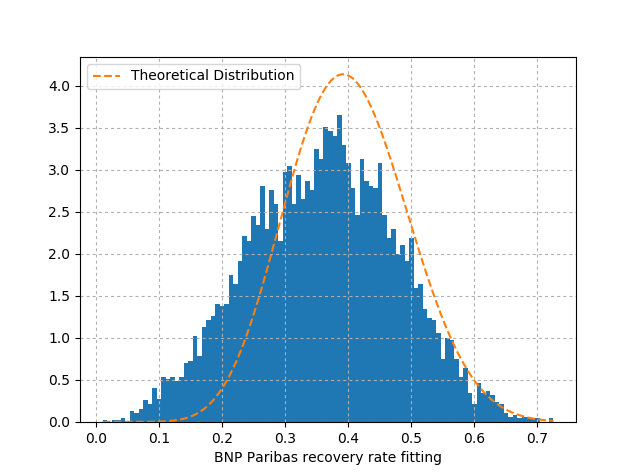
\includegraphics[scale=0.5]{bnp_fitting.png}
%				\caption{Simulated distribution of BNP Paribas recovery rate under the baseline calibration.}	
%			\end{figure}
%\end{frame}
 
%\subsection{Alternative balance-sheet calibration}
%
%\begin{frame}
%\frametitle{Alternative balance-sheet calibration: Introduction}
%
%While calibrating the NIG parameters to liquid option prices, within the described structural approach an alternative "ecomically sounding" experiment could be computing the relevant barrier triggers by relating them to some balance-sheet data. \\~\\
%
%One attempt to rely on accounting data would be to access to the last published balance-sheets\footnote{Source: https://it.finance.yahoo.com} and exploit a particularly successful practical implementation of structural credit modeling, i.e. the \textbf{KMV approach}. \\~\\
%
%Typically, in the KMV the trigger is given by the full short term liabilities plus half of the long term liabilities.
%
%
%\end{frame}
%
%
%	
%
%
%
%
%
%\begin{frame}
%\frametitle{Alternative balance-sheet calibration: results}
%\footnotesize{
%\begin{tabular}{ |p{2 cm}||p{1 cm}|p{1.6 cm}|p{1.1cm}|p{1cm}|p{1.3cm}|p{1.2 cm}| }
%	\hline
%	\multicolumn{7}{|c|}{\textbf{Alternative Counterparty Risk Value Adjustments }} \\
%	\hline
%	Contract type & $V_{0}$ & CVA  &CVA/$V_{0}$& DVA & DVA/$V_{0}$ &$\hat{V}_{0}$\\
%	\hline
%	Call Oil &5.82103 & 1.78212 &3061.527 &0 &0 &4.03890\\
%	Swap Gas &0.06716 &0.0011786 &175.092 &0 &0 & 0.06598\\
%	
%	\hline
%	
%\end{tabular}
%}
%
%The Table displays the results for the recomputed CCR metrics relative to a subset of the initial basket of energy commodity derivatives. \\~\\
%
%
%
%The effect of incorporating the alternative KMV-type calibration is the avoidance of any kind of DVA benefit for Enel since, the financial firm in the light of its accounting data, defaults first in all cases, making its experimental first-to-default probability within one year jump to about 41\%. As a consequence, CVA for Enel in both trades had roughly doubled.
%\end{frame}

\begin{frame}
\frametitle{Comments on stochastic recovery rates}
	In the light of my numerical results, I have observed that recovery rates seems to be responsible of some \textbf{leverage effect} on volatility: small mistakes in setting static recoveries imply large deviation from the actual implied volatilities.\\~\\

	I would \textbf{conclude} that neglecting the role of volatility and setting \textbf{flat recoveries} for all firms, in certain circumstances there configures some risk overestimation, as in the case of the corporate firm. 
	Conversely in other circumstances, there might configure some risk underestimation, as in the case of financial firm. The potential degree of \textbf{\emph{missing risk}} could be severe and might vanish the accuracy even of a sophisticated model.
\end{frame}

\begin{frame}
\Huge{\centerline{Thank you for attention!}}
\end{frame}


%\footnotesize{
%\begin{equation*}
%\pi_t = \mathbb{E}^{\mathbb{P}^{Dom} (t,T)}\left[ \frac{F^{Adj}(T) - K}{S(t)}\right]\mathbb{P}^{Dom} (t,T) - \mathbb{E}^{\mathbb{P}^{For} (t,T)}\left[ \frac{F(T)-K}{S(t)} \right]\mathbb{P}^{For} (t,T)	
%\end{equation*}}


%\begin{frame}[allowframebreaks]%in case more than 1 slide needed
%\frametitle{References}
%\bibliography{draft}
%\nocite{*}
%\bibliographystyle{chicago}
%\end{frame}


\end{document}